\documentclass[12pt,letterpaper]{article}
\usepackage[utf8]{inputenc}
\usepackage[spanish]{babel}
\usepackage{graphicx}
\usepackage[left=2cm,right=2cm,top=2cm,bottom=2cm]{geometry}
\usepackage{graphicx} % figuras
% \usepackage{subfigure} % subfiguras
\usepackage{float} % para usar [H]
\usepackage{amsmath}
%\usepackage{txfonts}
\usepackage{stackrel} 
\usepackage{multirow}
\usepackage{enumerate} % enumerados
\renewcommand{\labelitemi}{$-$}
\renewcommand{\labelitemii}{$\cdot$}
% \author{}
% \title{Caratula}
\begin{document}

% Fancy Header and Footer
% \usepackage{fancyhdr}
% \pagestyle{fancy}
% \cfoot{}
% \rfoot{\thepage}
%

% \usepackage[hidelinks]{hyperref} % CREA HYPERVINCULOS EN INDICE

% \author{}
\title{Caratula}

\begin{titlepage}
\begin{center}
\large{UNIVERSIDAD PRIVADA DE TACNA}\\
\vspace*{-0.025in}
\begin{figure}[htb]
\begin{center}

\includegraphics[width=8cm]{./Imagenes/logo}
\end{center}
\end{figure}
\vspace*{0.15in}
INGENIERIA DE SISTEMAS  \\

\vspace*{0.5in}
\begin{large}
TITULO:\\
\end{large}

\vspace*{0.1in}
\begin{Large}
\textbf{INFORME DE LABORATORIO 02} \\
\end{Large}

\vspace*{0.3in}
\begin{Large}
\textbf{CURSO:} \\
\end{Large}

\vspace*{0.1in}
\begin{large}
INTELIGENCIA DE NEGOCIOS\\
\end{large}

\vspace*{0.3in}
\begin{Large}
\textbf{DOCENTE(ING):} \\
\end{Large}

\vspace*{0.1in}
\begin{large}
 Patrick Cuadros Quiroga\\
\end{large}

\vspace*{0.2in}
\vspace*{0.1in}
\begin{large}
Integrantes: \\
\begin{flushleft}


Mamani Ayala, Brandon     \hfill	(2015052715) \\

\end{flushleft}
\end{large}
\end{center}

\end{titlepage}


\tableofcontents % INDICE
\thispagestyle{empty} % INDICE SIN NUMERO
\newpage
\setcounter{page}{1} % REINICIAR CONTADOR DE PAGINAS DESPUES DEL INDICE

\section{Desarrollo} 


\begin{itemize}
\item Tarea 1 : Relaciones automaticas


\begin{enumerate}
\item Inciar Power BI Desktop

\begin{center}
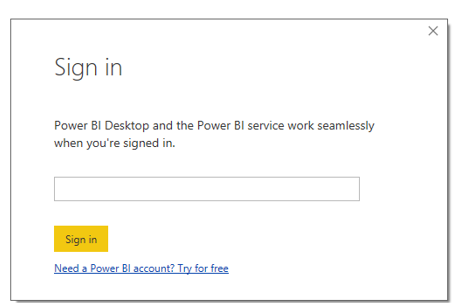
\includegraphics[scale=0.55]{./Imagenes/a1.png}
\end{center}

\item En la Ventana de Power BI Desktop, click en Obtener Datos (Get Data) . Seguidamente en el cuadro de dialogos Obtener Datos (Get Data), asegurarse que Excel esta seleccionado y hacer clicken Conectar (Connect).

\begin{center}
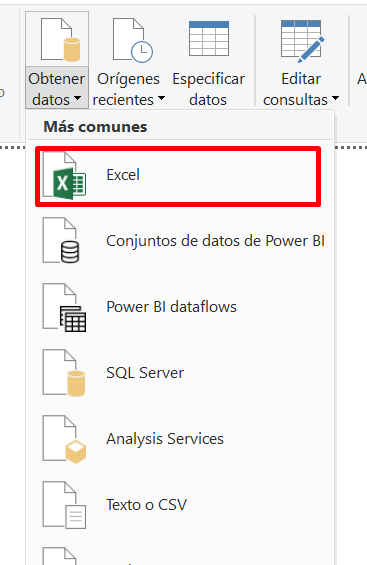
\includegraphics[scale=0.55]{./Imagenes/a2.png}
\end{center}

\item En el cuadro de dialogo Abrir (Open), buscar el archivo Adventure Works Sales Data.xlsx, y luego hacer click en Abrir (Open).

\begin{center}
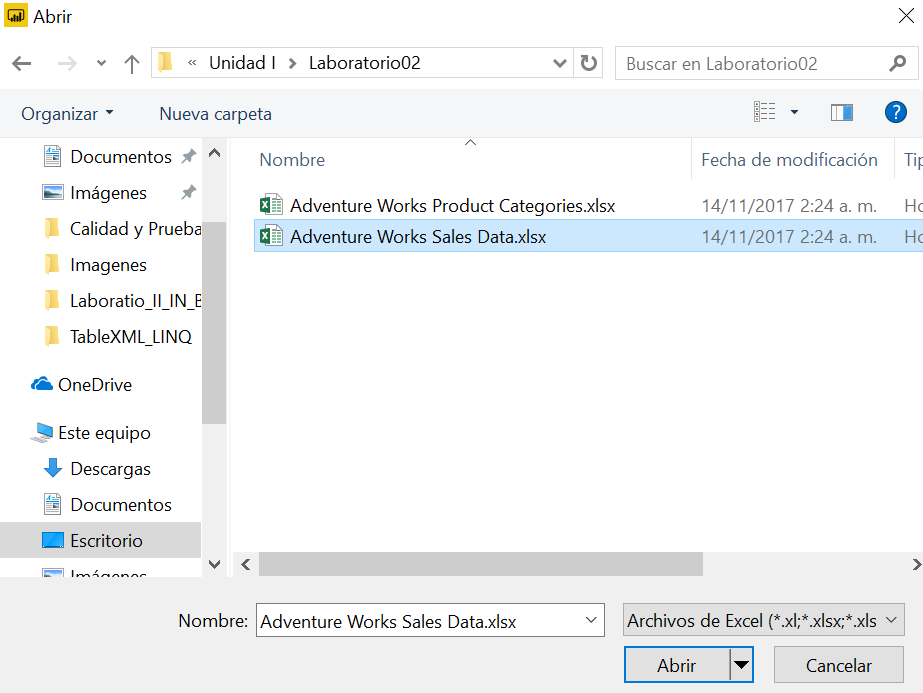
\includegraphics[scale=0.55]{./Imagenes/a4.png}
\end{center}


\item En el cuadro de dialogo base de datos SQL Server, en la casilla servidor tipear (local), en la casilla Base de datos (opcional) / Database (optional), tipear AdventureWorks2017, y hacer clic en OK.

\begin{center}
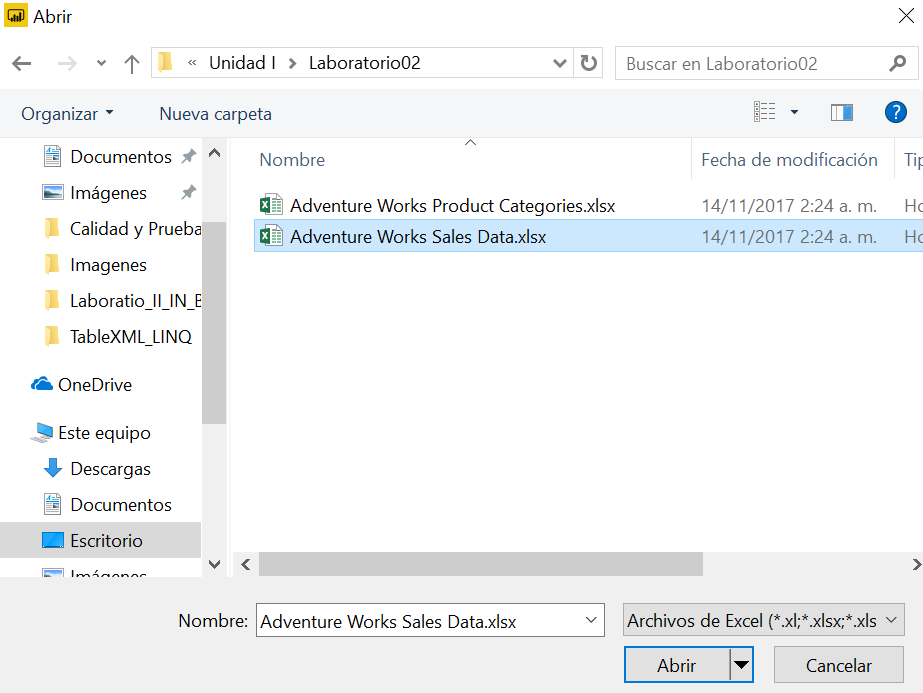
\includegraphics[scale=0.55]{./Imagenes/a4.png}
\end{center}

\item En el cuadro de dialogo Explorador (Navigator), seleccionar las hojas DimCurrency, DimCustomer, DimDate, DimProduct, DimPromotion, DimSalesTerritory, y FactInternetSales. 

\begin{center}
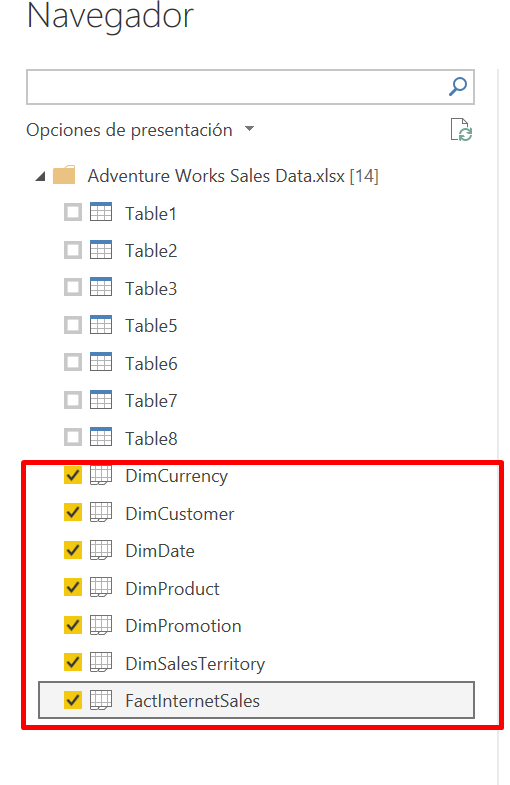
\includegraphics[scale=0.55]{./Imagenes/a3.png}
\end{center}

\item Hacer click en Cargar (Load).
\begin{center}
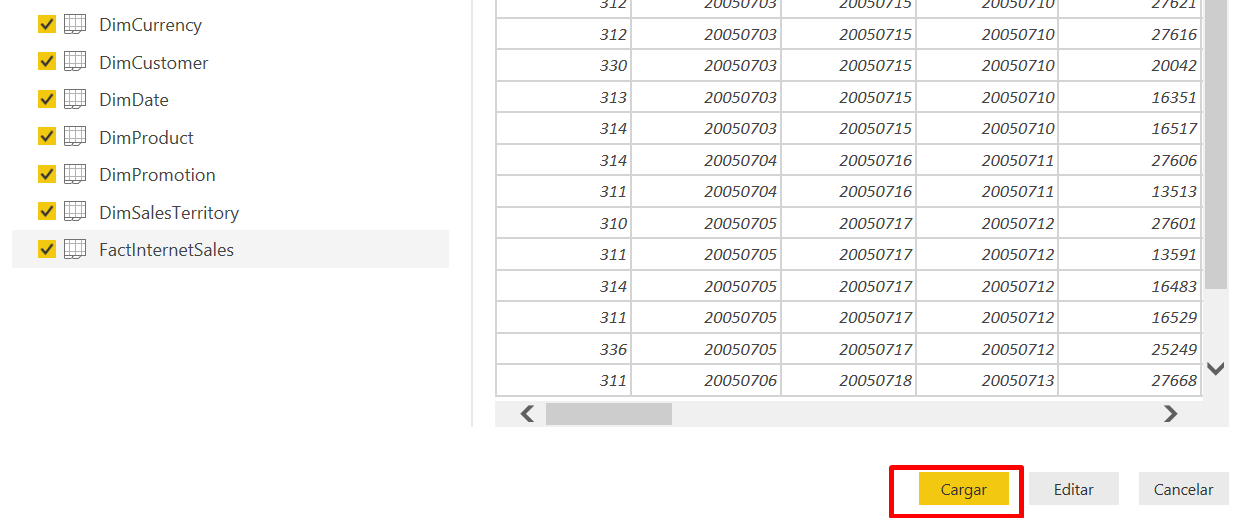
\includegraphics[scale=0.55]{./Imagenes/a5.png}
\end{center}

\item En el menú principal, hacer click en Administrar relaciones (Manage Relationships).

\begin{center}
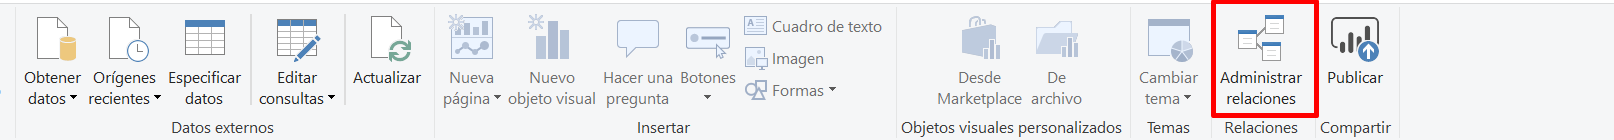
\includegraphics[scale=0.55]{./Imagenes/17.png}
\end{center}

\item En el cuadro de Administrar relaciones (Manage Relationships), hacer click en Nueva (New)

\begin{center}

\includegraphics[scale=0.55]{./Imagenes/new.png}
\end{center}


\item En el cuadro de Administrar relaciones (Manage Relationships), en la lista de tablas superior, hacer click en FactInternetSales. 

\begin{center}
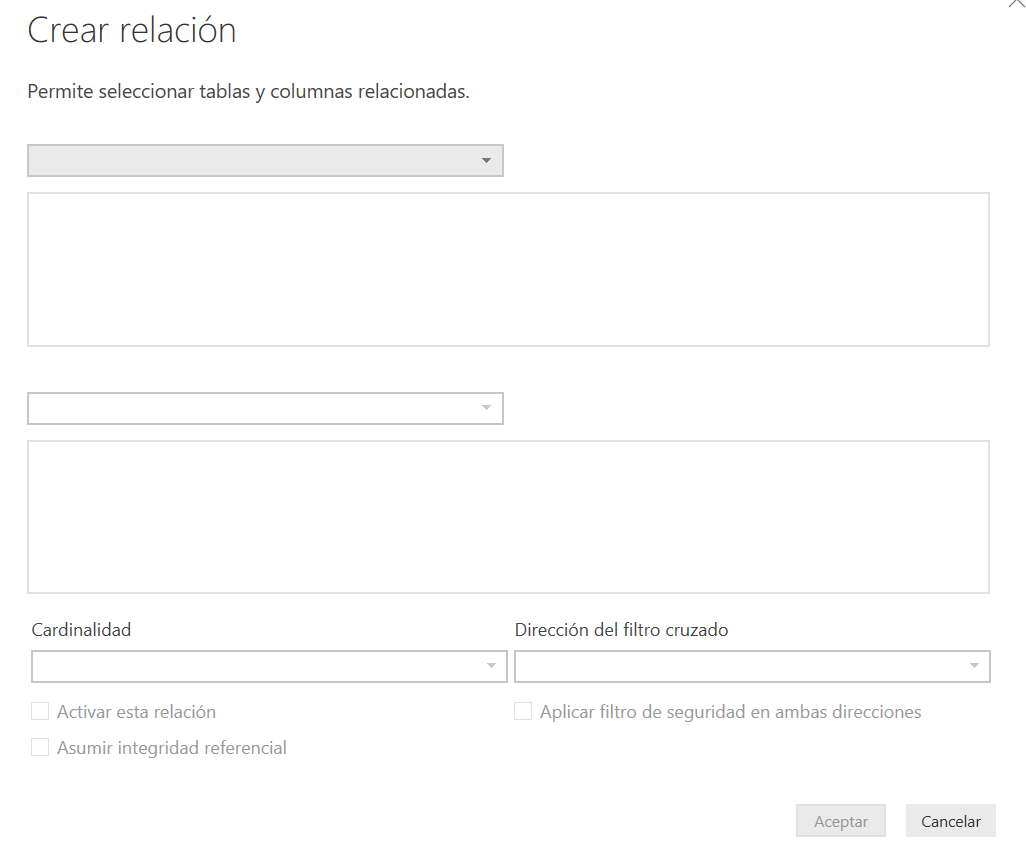
\includegraphics[scale=0.55]{./Imagenes/9.png}
\end{center}

\item Cuando la vista previa de la table aparezca hacer click en la columna OrderDateKey.

\begin{center}
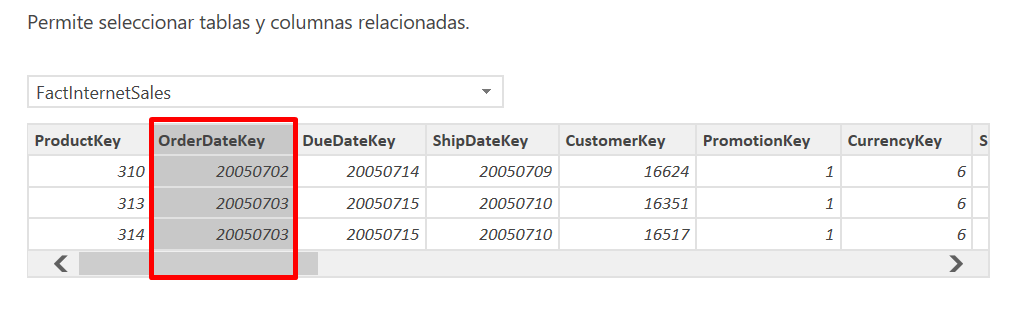
\includegraphics[scale=0.55]{./Imagenes/10.png}
\end{center}

\item En la lista de table inferior, hacer click en DimDate. Cuando la vista previa de la table aparezca hacer click en la columna DateKey.

\begin{center}
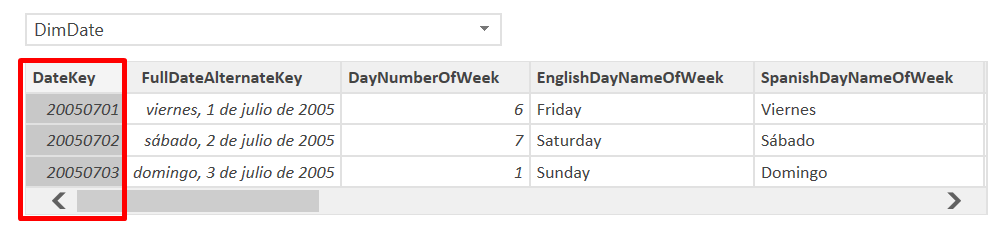
\includegraphics[scale=0.55]{./Imagenes/11.png}
\end{center}

\item Revisar que la cardinalidad (Cardinality) esta seleccionada para Muchos a Uno (Many to One (*:1)), que la Dirección del filtro cruzado (Cross filter direction) es Sencilla (Single), y que la opción Hacer esta relación activa (Make this relationship active) se encuentra seleccionada, luego hacer click en Aceptar (OK).

\begin{center}
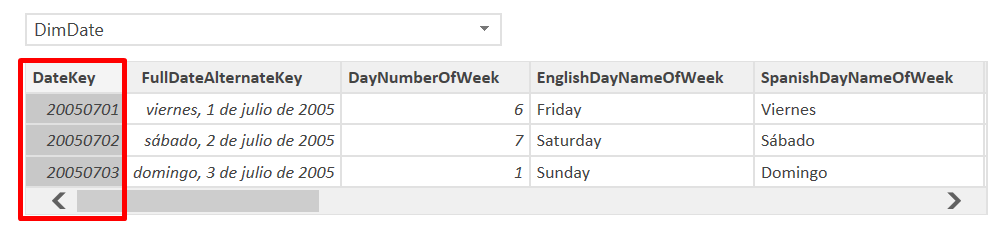
\includegraphics[scale=0.55]{./Imagenes/11.png}
\end{center}

\item En el cuadro de Administrar relaciones (Manage Relationships), hacer click en Cerrar (Close)

\begin{center}
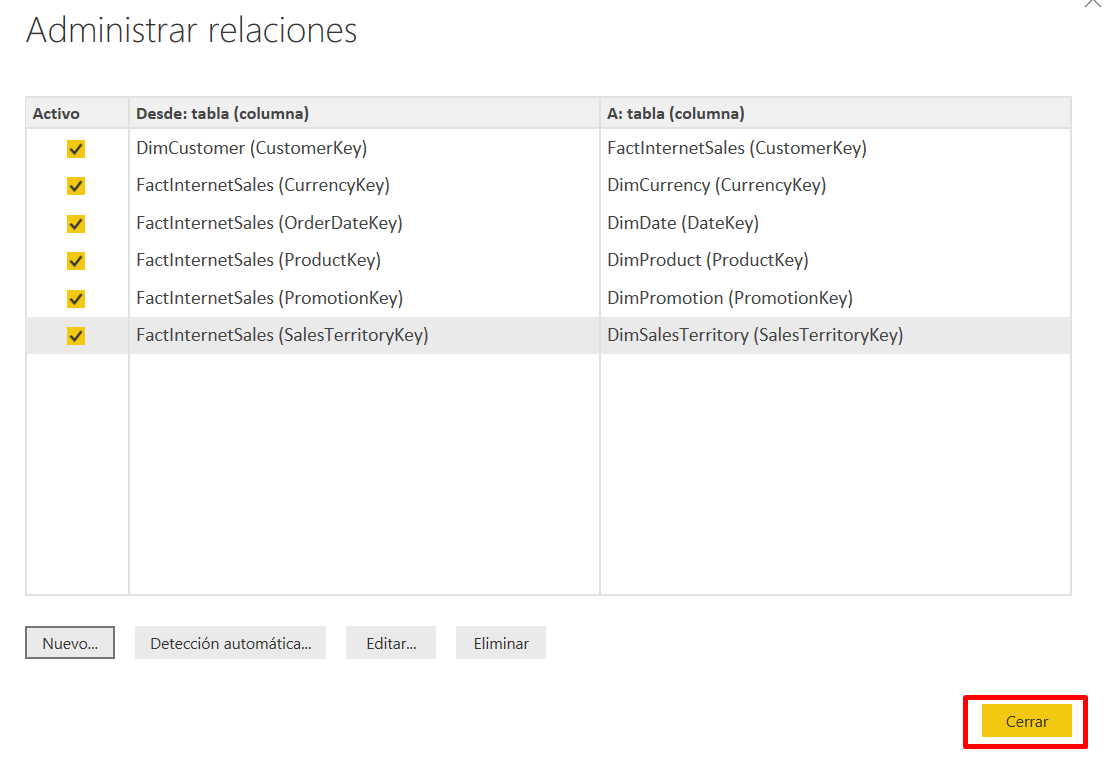
\includegraphics[scale=0.55]{./Imagenes/13.png}
\end{center}

\item En el diagrama, en la tabla FactInternetSales, hacer click en la columna DueDateKey.Arrastrar la columna DueDateKey a la columna DateKey de la tabla DimDate

\begin{center}
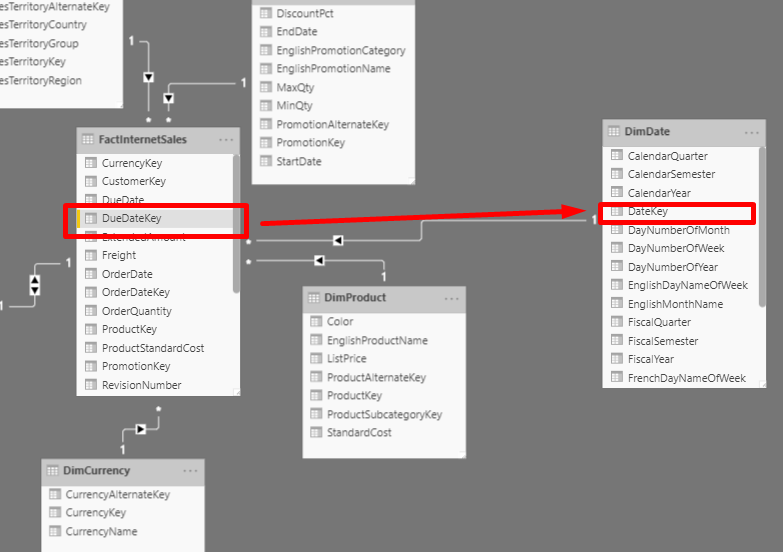
\includegraphics[scale=0.55]{./Imagenes/15.png}
\end{center}

\item En el diagrama, en la tabla FactInternetSales, hacer click en la columna ShipDateKey. Arrastrar la columna ShipDateKey a la columna DateKey de la tabla DimDate.


\begin{center}
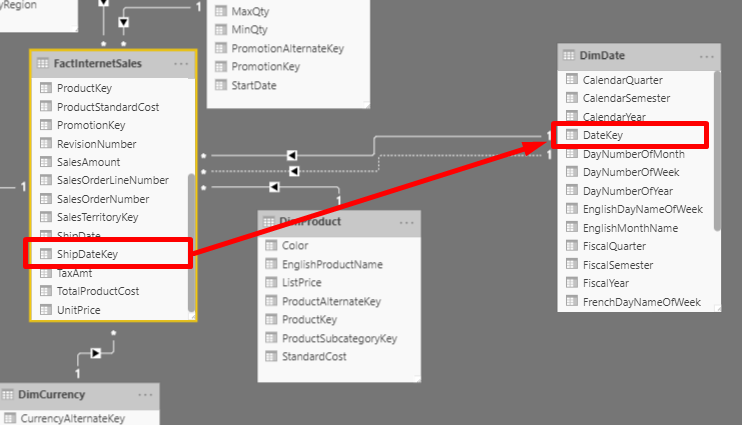
\includegraphics[scale=0.55]{./Imagenes/16.png}
\end{center}

\item En el menú principal, hacer click en Administrar relaciones (Manage Relationships)

\begin{center}
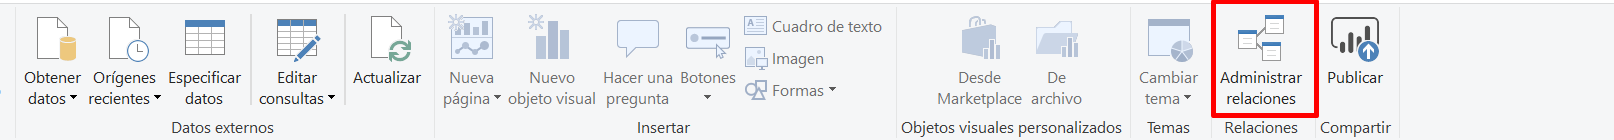
\includegraphics[scale=0.55]{./Imagenes/17.png}
\end{center}


\item En el cuadro de Administrar relaciones (Manage Relationships), hacer doble click en la relación FactInternetSales (CurrencyKey)

\begin{center}
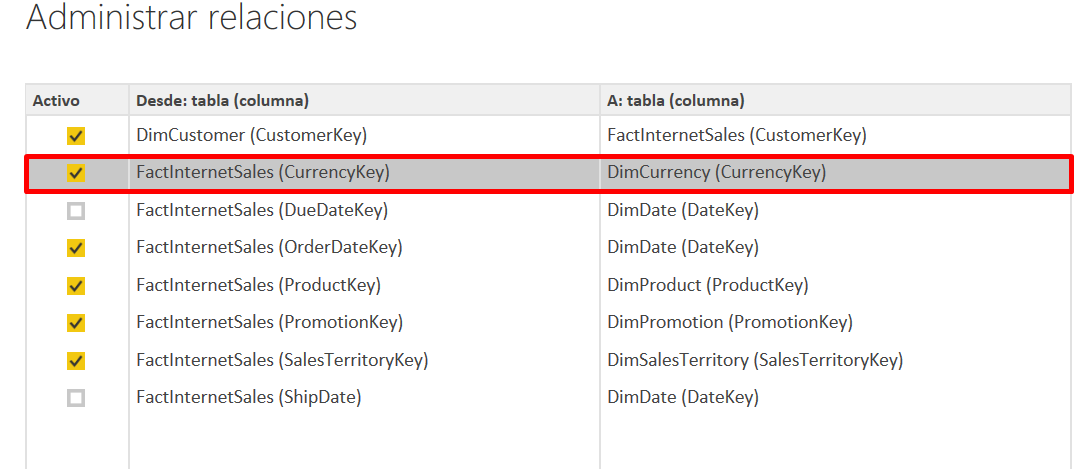
\includegraphics[scale=0.55]{./Imagenes/18.png}
\end{center}

\item  En la lista de Dirección de Filtro Cruzado (Cross filter direction), hacer click en Sencilla (Single), luego hacer click en Aceptar (OK)

\begin{center}
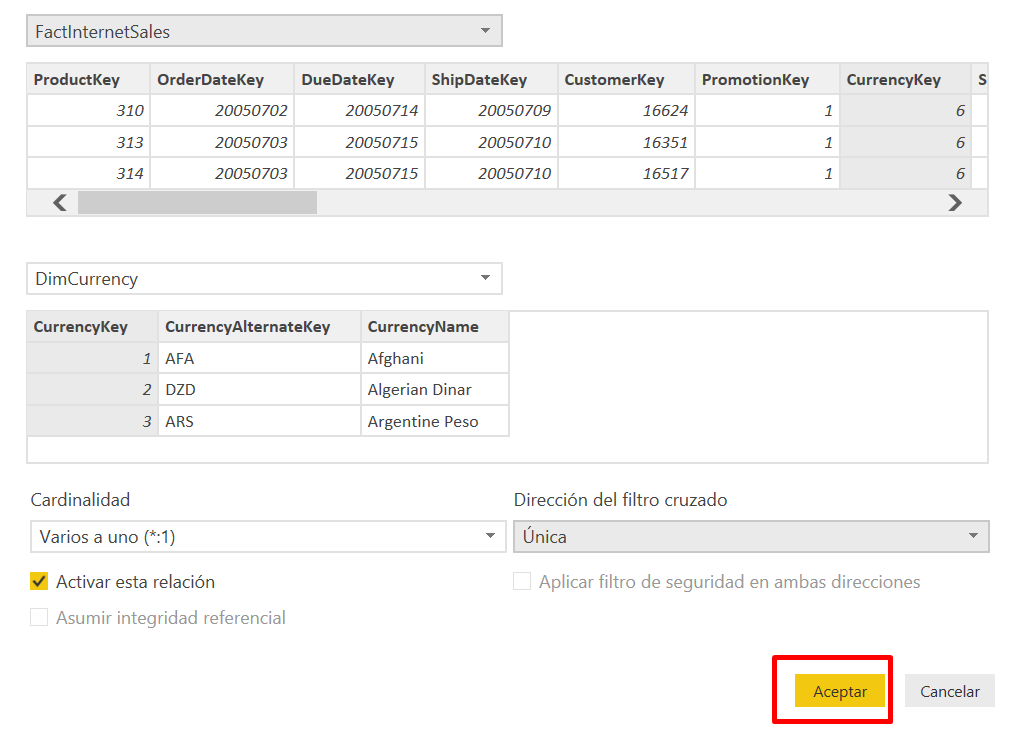
\includegraphics[scale=0.55]{./Imagenes/19.png}
\end{center}

\item En el cuadro de Administrar relaciones (Manage Relationships), hacer doble click en la relación FactInternetSales (ProductKey).

\begin{center}
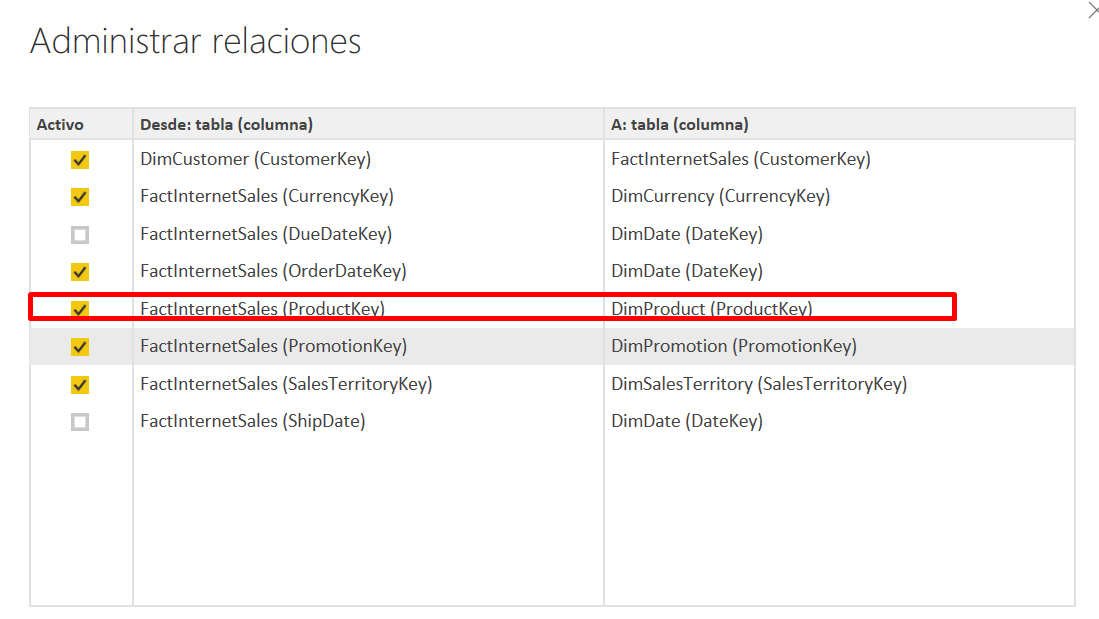
\includegraphics[scale=0.55]{./Imagenes/22.png}
\end{center}

\item En la lista de Dirección de Filtro Cruzado (Cross filter direction), hacer click en Sencilla (Single), luego hacer click en Aceptar (OK).

\begin{center}
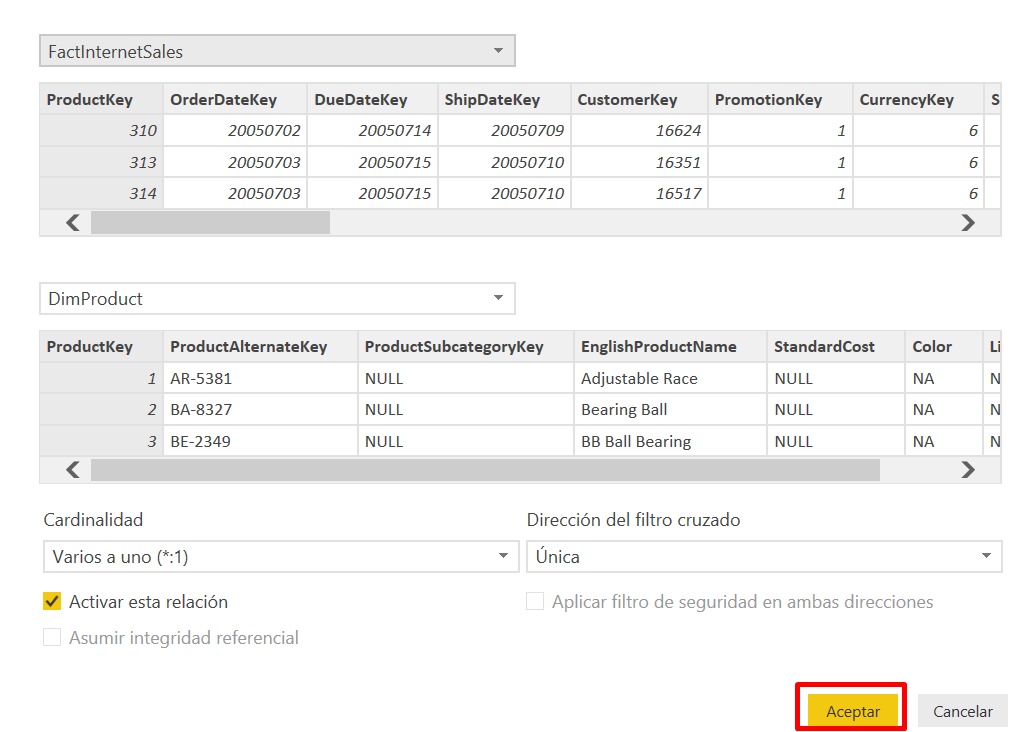
\includegraphics[scale=0.55]{./Imagenes/20.png}
\end{center}

\item En el cuadro de Administrar relaciones (Manage Relationships), hacer doble click en la relación FactInternetSales (PromotionKey).


\begin{center}
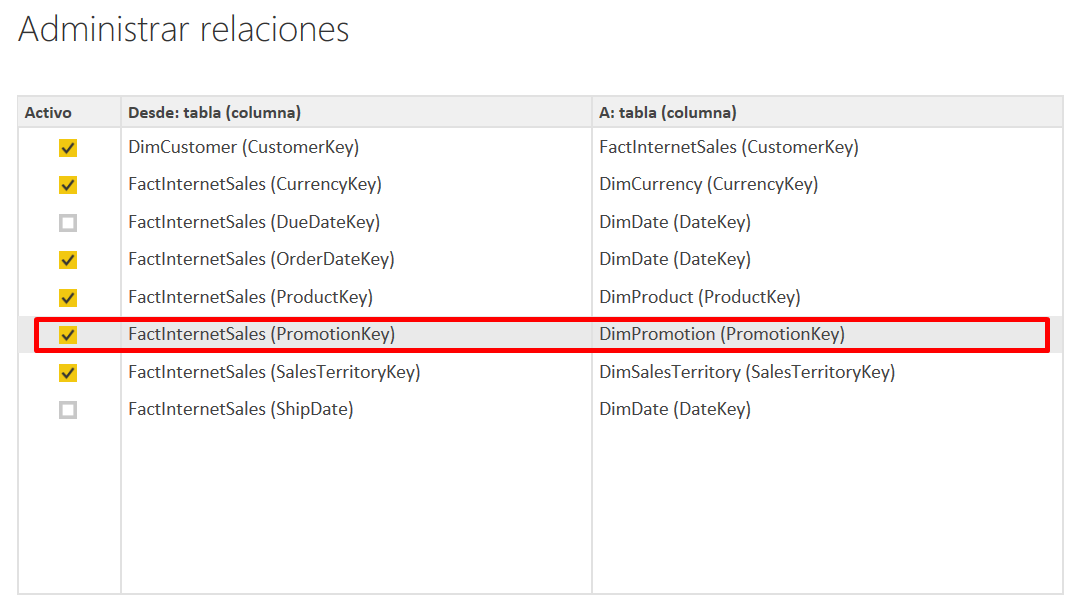
\includegraphics[scale=0.55]{./Imagenes/21.png}
\end{center}

\item . En la lista de Dirección de Filtro Cruzado (Cross filter direction), hacer click en Sencilla (Single), luego hacer click en Aceptar (OK).

\begin{center}
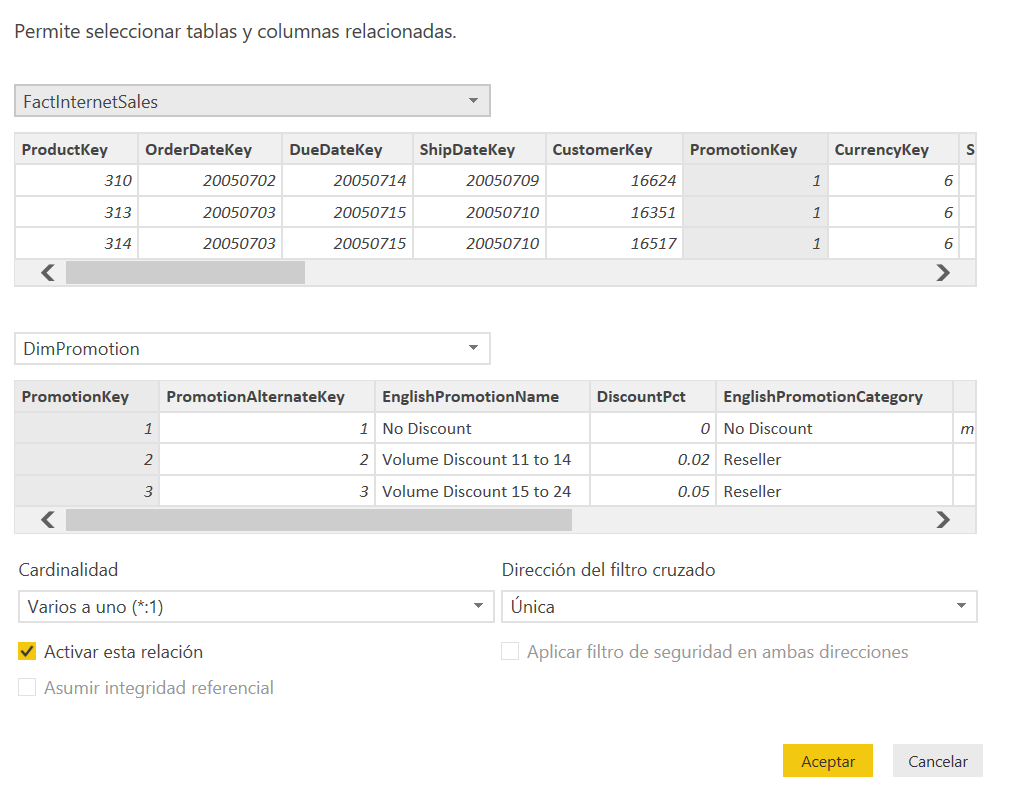
\includegraphics[scale=0.55]{./Imagenes/23.png}
\end{center}

\item En el cuadro de Administrar relaciones (Manage Relationships), hacer doble click en la relación FactInternetSales (SalesTerritoryKey).

\begin{center}
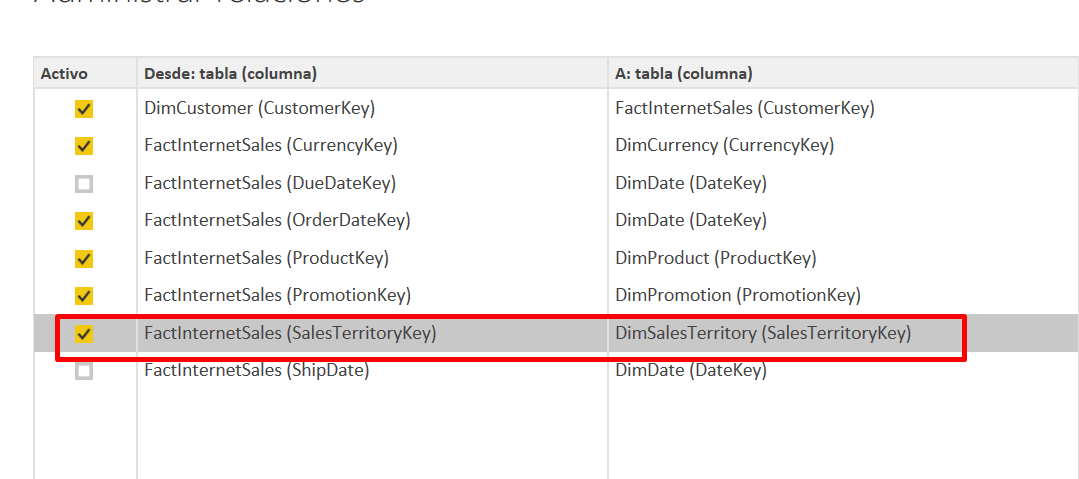
\includegraphics[scale=0.55]{./Imagenes/24.png}
\end{center}

\item En la lista de Dirección de Filtro Cruzado (Cross filter direction), hacer click en Sencilla (Single), luego hacer click en Aceptar (OK).

\begin{center}
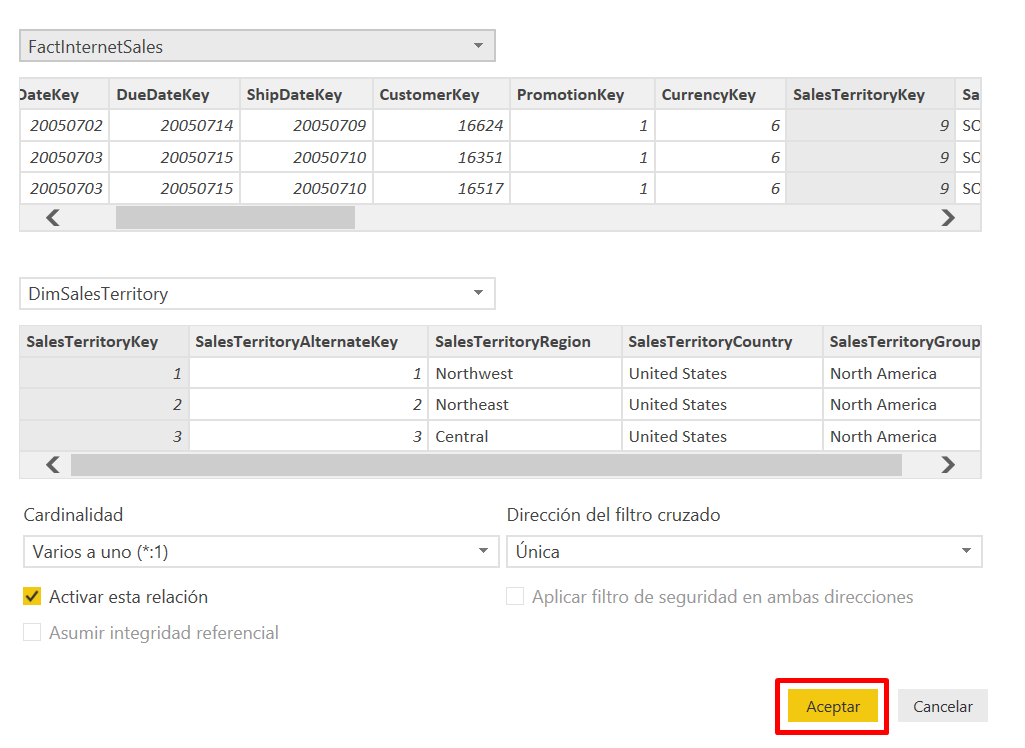
\includegraphics[scale=0.55]{./Imagenes/25.png}
\end{center}


\item En el cuadro de Administrar relaciones (Manage Relationships), hacer click en Cerrar (Close).

\begin{center}
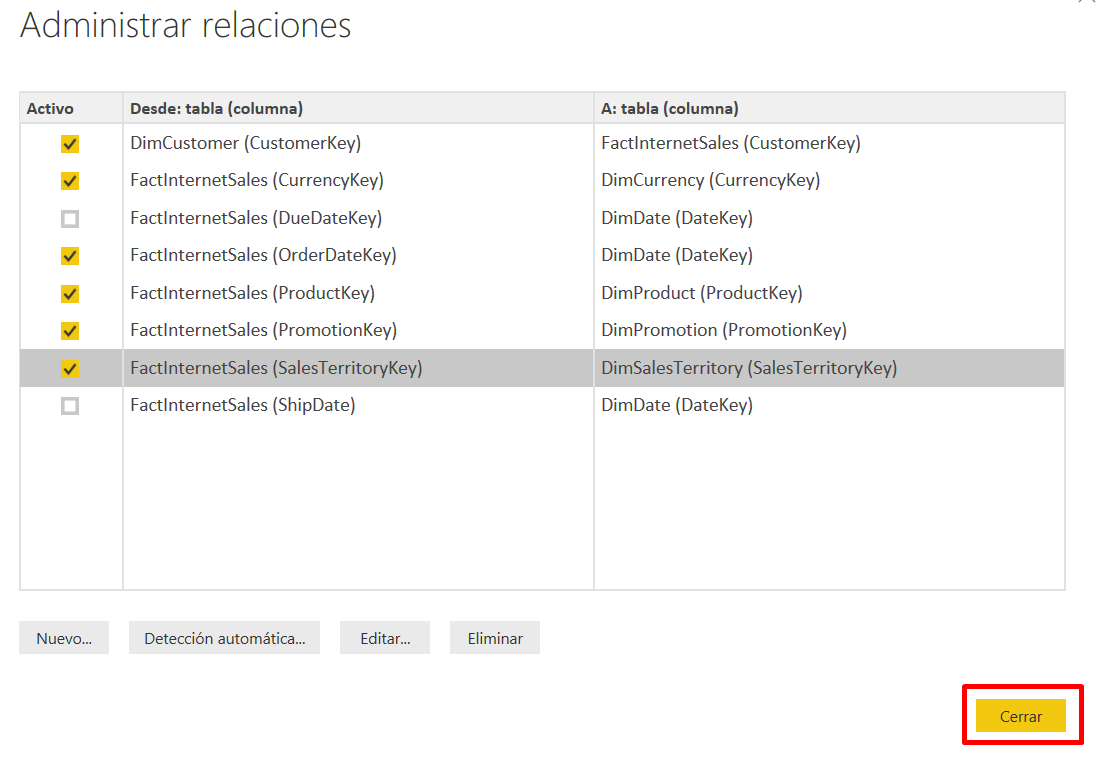
\includegraphics[scale=0.55]{./Imagenes/26.png}
\end{center}

\item Hacer click en la línea de relación entre FactInternetSales and DimCustomer y presionar Borrar (Delete).

\begin{center}
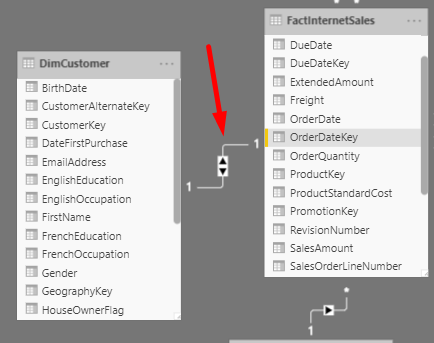
\includegraphics[scale=0.55]{./Imagenes/27.png}
\end{center}

\item En el cuadro de dialogo Eliminar relación (Delete Relationship), hacer click en Borrar (Delete).


\begin{center}
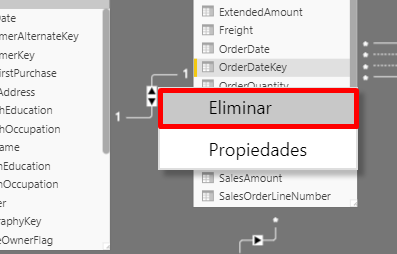
\includegraphics[scale=0.55]{./Imagenes/28.png}
\end{center}

\item . En el cuadro de dialogo Eliminar relación (Delete Relationship), hacer click en Borrar (Delete).

\begin{center}
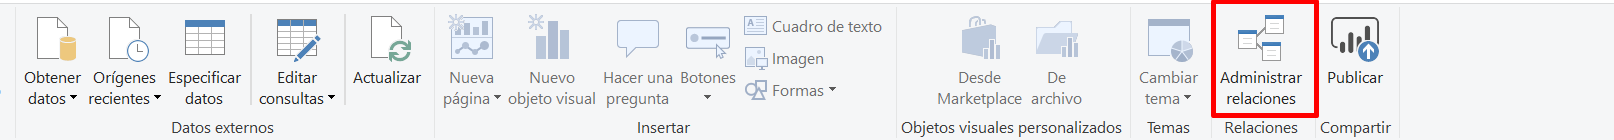
\includegraphics[scale=0.55]{./Imagenes/17.png}
\end{center}

\item En el cuadro de Administrar relaciones (Manage Relationships), hacer click en Nueva (New).

\begin{center}
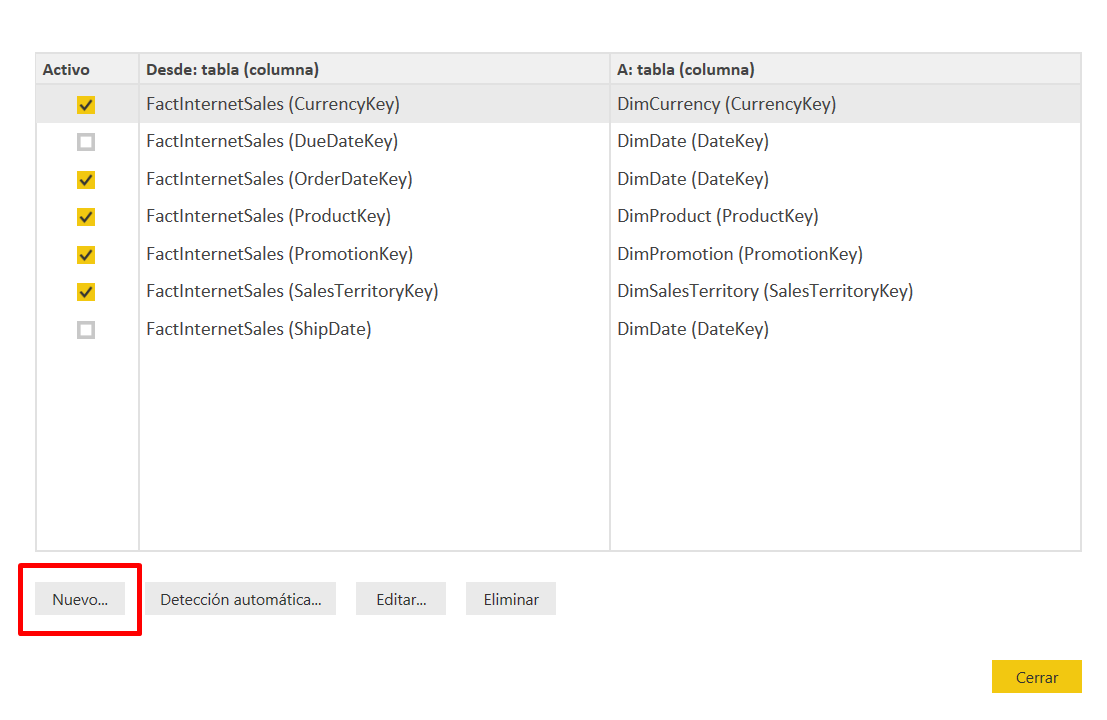
\includegraphics[scale=0.55]{./Imagenes/29.png}
\end{center}

\item En la lista de tablas superior, hacer click en FactInternetSales. Luego hacer click en la columna CustomerKey en la vista de datos previa

\begin{center}
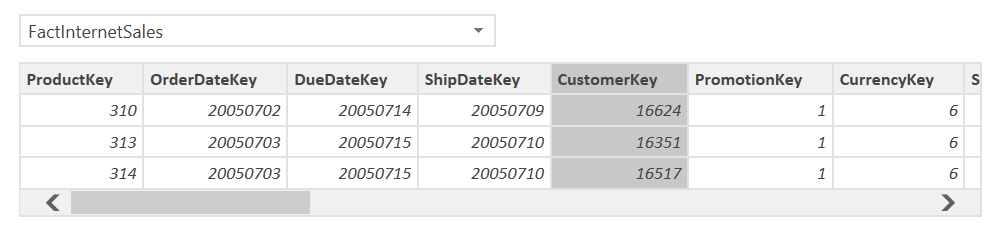
\includegraphics[scale=0.55]{./Imagenes/30.png}
\end{center}

\item En la lista de tablas superior, hacer click en DimCustomer, y hacer click CustomerKey en la vista de datos previa.

\begin{center}
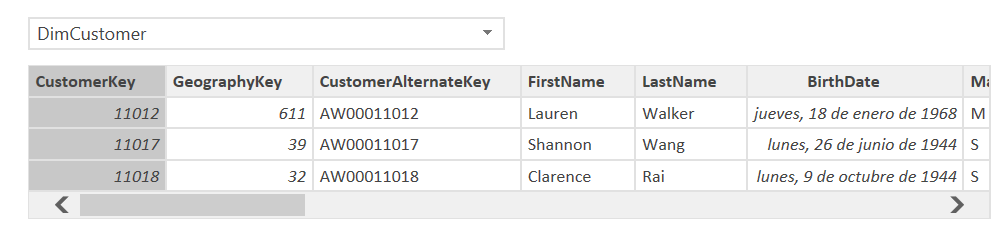
\includegraphics[scale=0.55]{./Imagenes/31.png}
\end{center}

\item En la lista de Cardinalidad (Cardinality), hacer click en Muchos a Uno (Many to One (*:1)), y luego hacer click en Aceptar (OK).

\begin{center}
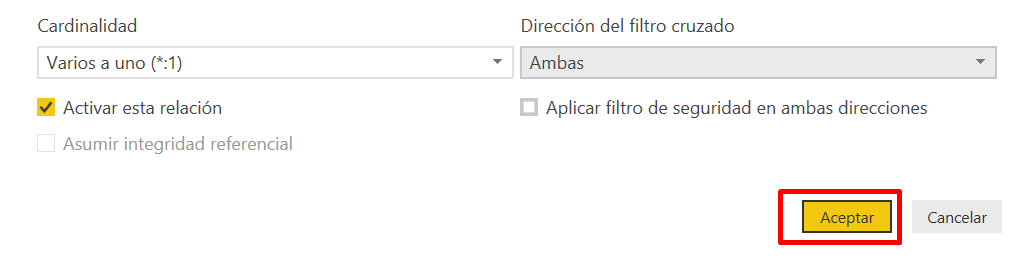
\includegraphics[scale=0.55]{./Imagenes/32.png}
\end{center}


\item Hacer click en Guardar (Save), y cuargar el archive como Ventas Adventure Works.pbix.

\begin{center}
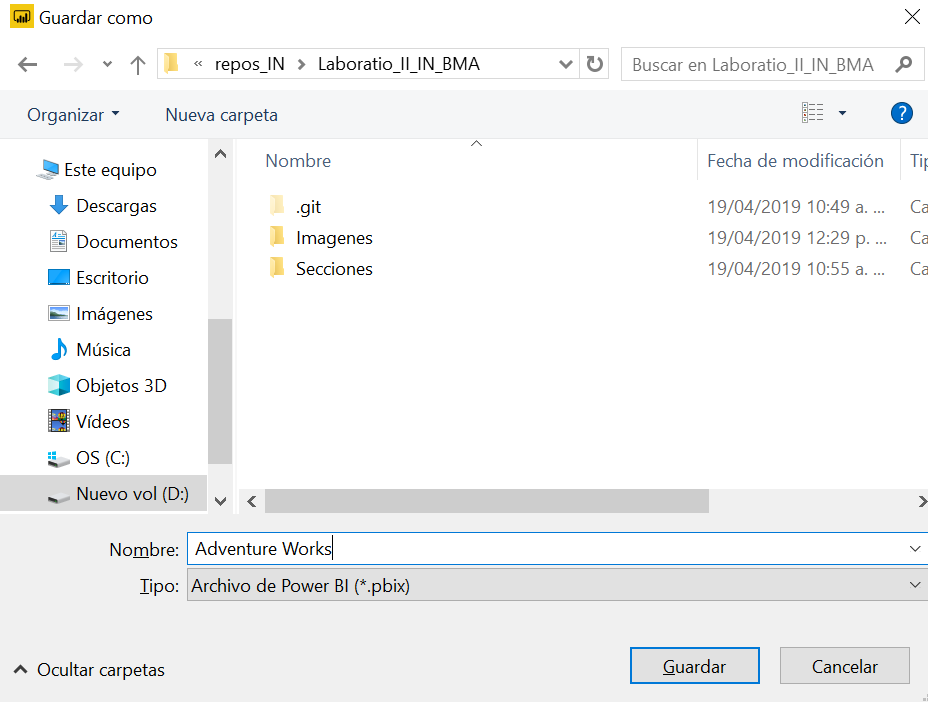
\includegraphics[scale=0.55]{./Imagenes/33.png}
\end{center}

\end{enumerate}



\item Tarea 2 : Relaciones Manuales
\begin{enumerate}

\item En la Ventana de Power BI Desktop, click en Obtener Datos (Get Data) y luego en Excel.

\begin{center}
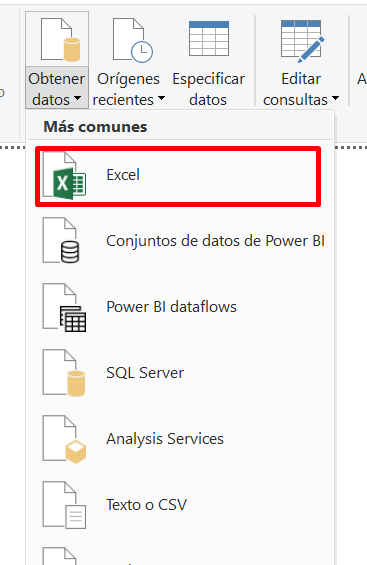
\includegraphics[scale=0.55]{./Imagenes/a2.png}
\end{center}


\item Abrir el archivo Adventure Works Product Categories.xlsx.
\begin{center}
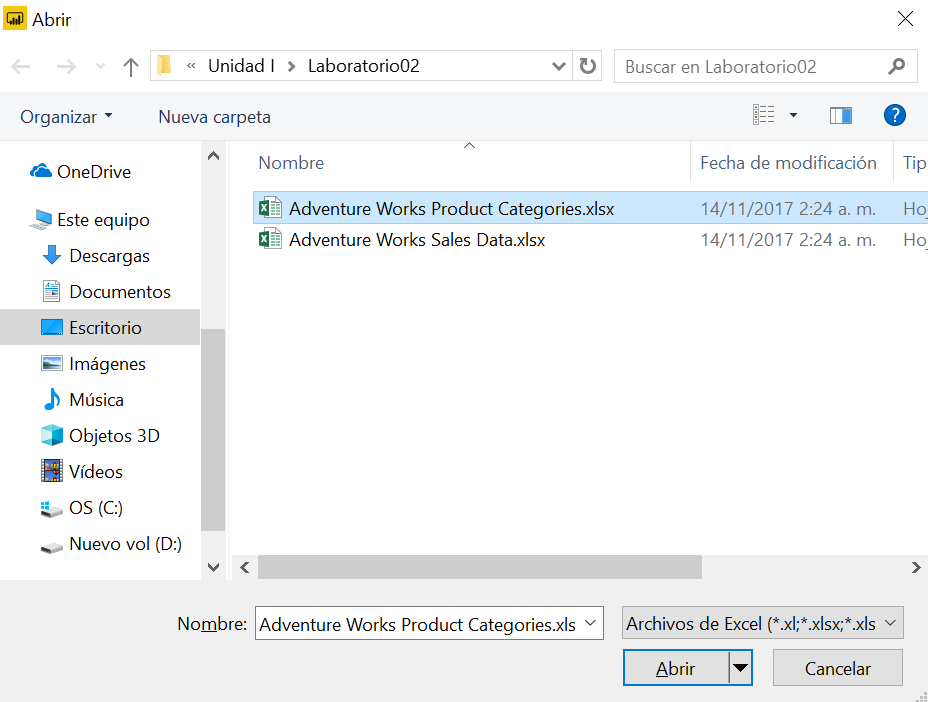
\includegraphics[scale=0.55]{./Imagenes/b2.png}
\end{center}

\item En el cuadro de dialogo Explorador (Navigator), seleccionar las hojas DimProductCategory, and DimProductSubcategory, y luego hacer click en Cargar (Load).
\begin{center}
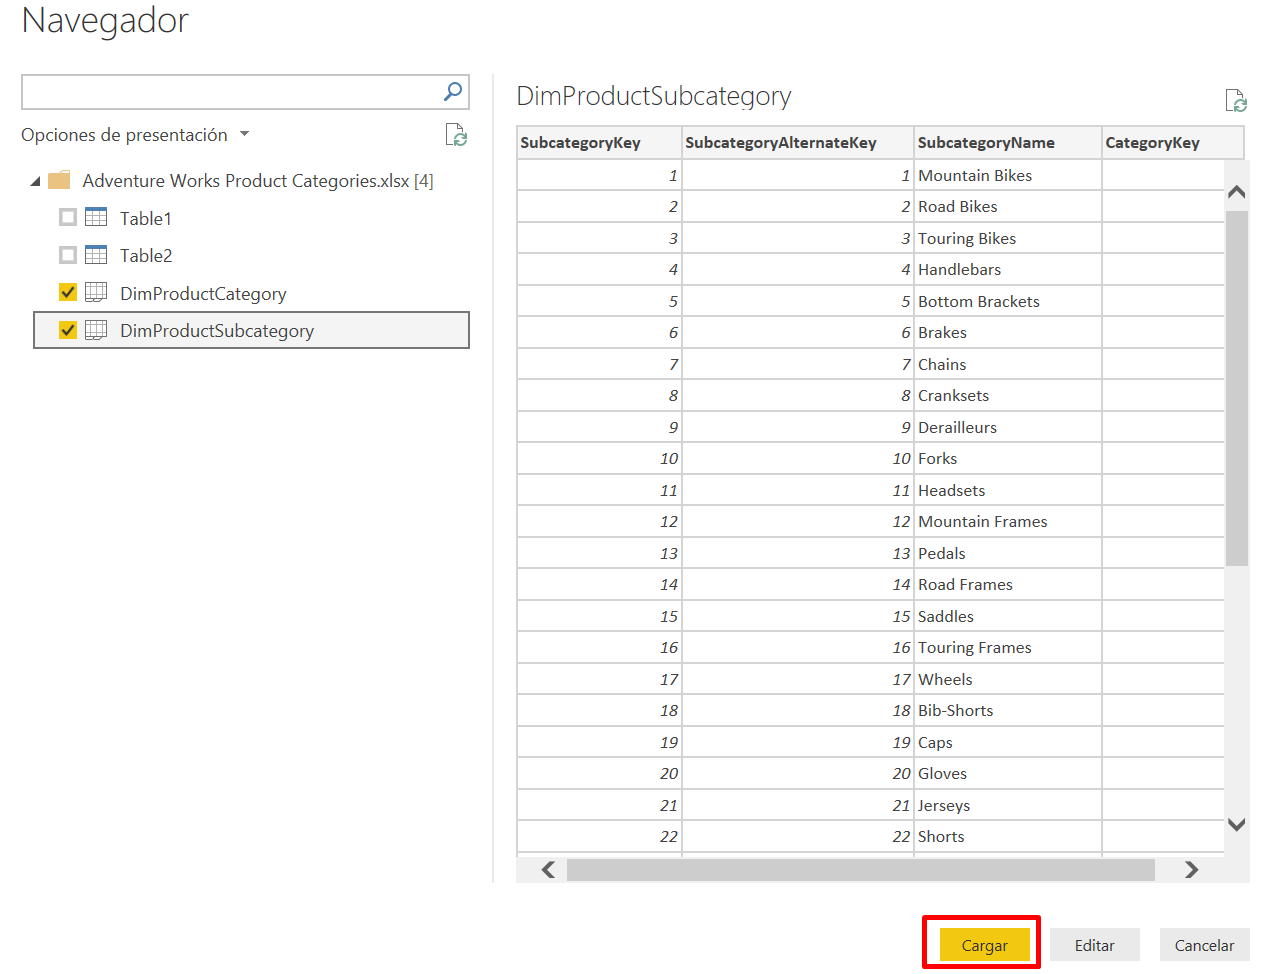
\includegraphics[scale=0.55]{./Imagenes/b3.png}
\end{center}

\item En el panel de Relaciones, revisar la relación que Power BI ha creado entre las dos tablas.
\begin{center}
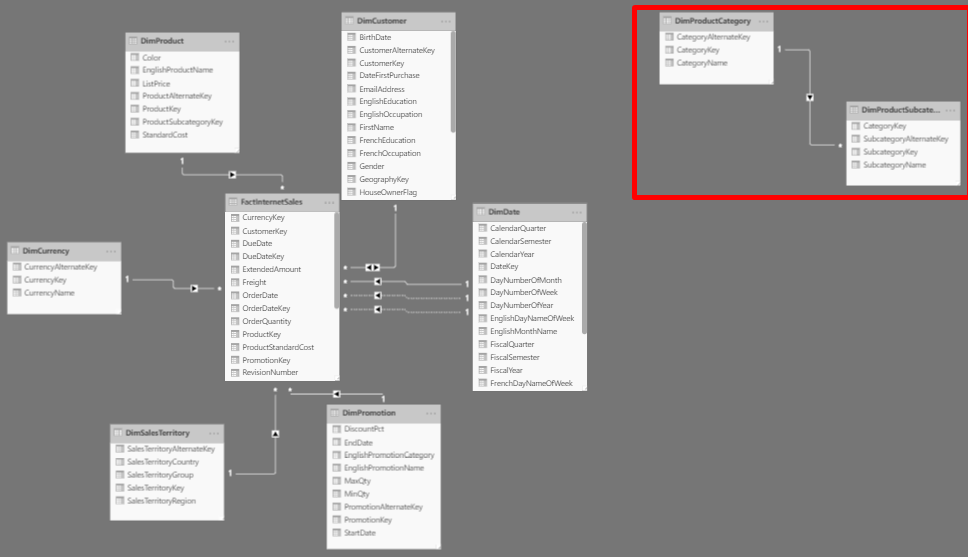
\includegraphics[scale=0.55]{./Imagenes/b4.png}
\end{center}

\item . Hacer click en la línea de la relación entre DimProductCategory, y DimProductSubcategory, y seleccionar Eliminar (Delete).
\begin{center}
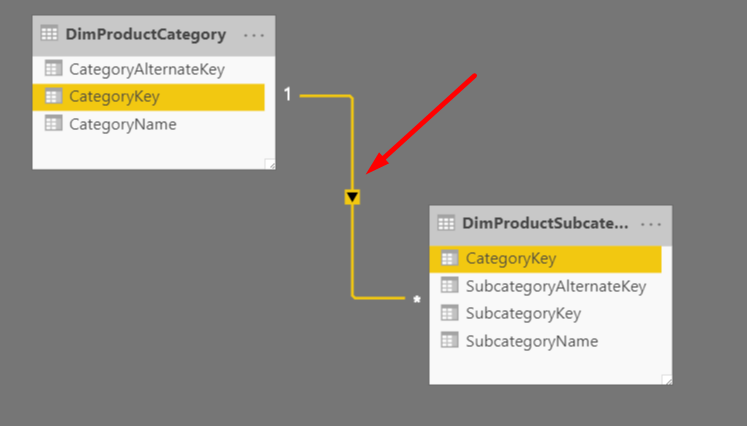
\includegraphics[scale=0.55]{./Imagenes/b5.png}
\end{center}

\item En el cuadro de dialogo Eliminar relación (Delete Relationship), hacer click en Borrar (Delete).
\begin{center}
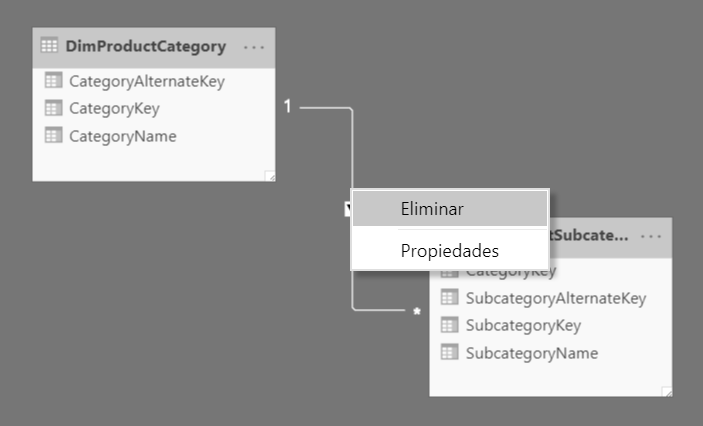
\includegraphics[scale=0.55]{./Imagenes/b6.png}
\end{center}

\item Arrastrar la columna CategoryKey en la tabla DimProductSubcategory a la columna Category en la tabla DimProductCategory, para crear una relación Muchos a uno (Many to One (*:1)), y una dirección de filtro cruzado (Cross filter direction) en ambos.
\begin{center}
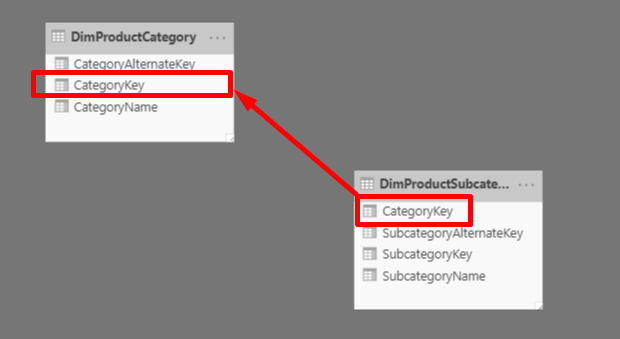
\includegraphics[scale=0.55]{./Imagenes/b7.png}
\end{center}

\begin{center}
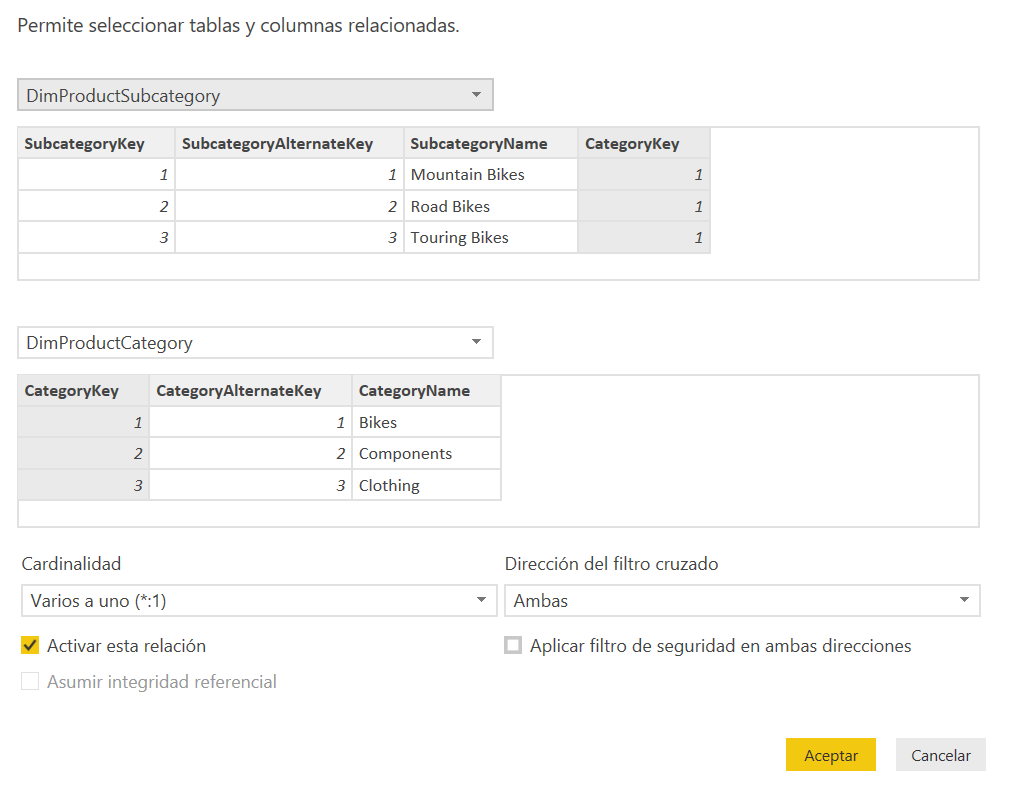
\includegraphics[scale=0.55]{./Imagenes/b8.png}
\end{center}

\item En la tabla DimProduct, arrastrar la columna ProductSubcategoryKey a la columna SubcategoryKey en la tabla DimProductSubcategory, para crear una relación de Muchos a Uno (Many to One (*:1)), y una dirección de filtro cruzado (Cross filter direction) en ambos.
\begin{center}
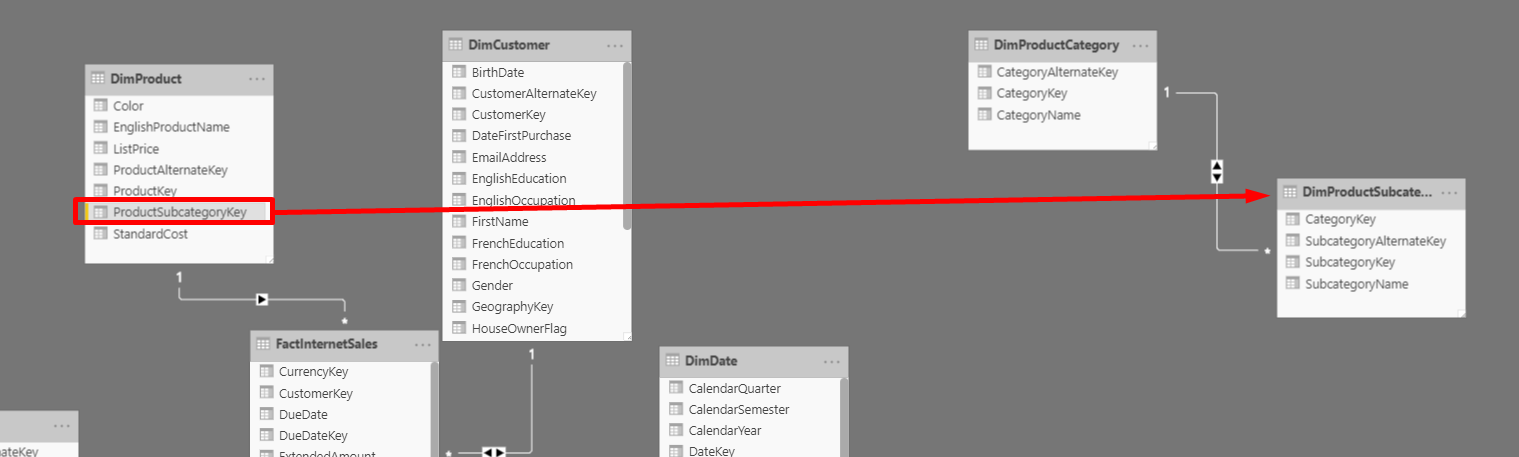
\includegraphics[scale=0.55]{./Imagenes/b9.png}
\end{center}

\begin{center}
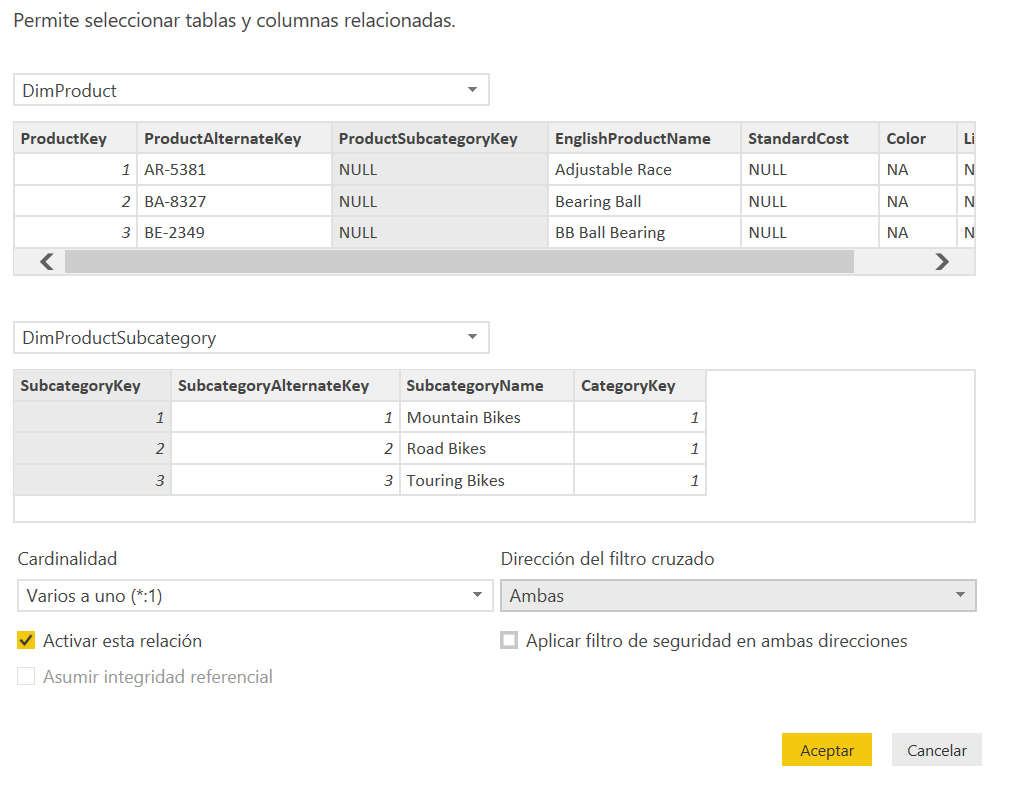
\includegraphics[scale=0.55]{./Imagenes/b10.png}
\end{center}

\item Hacer click en Guardar
\begin{center}
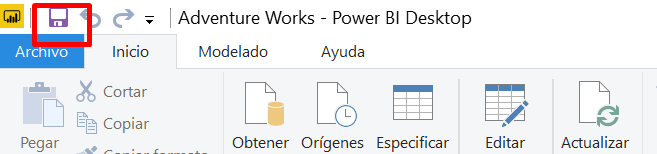
\includegraphics[scale=0.55]{./Imagenes/b11.png}
\end{center}

\end{enumerate}



\end{itemize}







 	 	


\end{document}
